\chapter{Zakłócenie w regulatorze DMC}
\label{zad5}
Poniżej (rys. \ref{fig:zak_bezr}) został zaprezentowany przebieg, w którym po osiągnięciu wartości zadanej, w chwili $k=100$ następuje skokowy wzrost zakłócenie z $0$ na $1$.

\begin{figure}[h!]
	\centering
	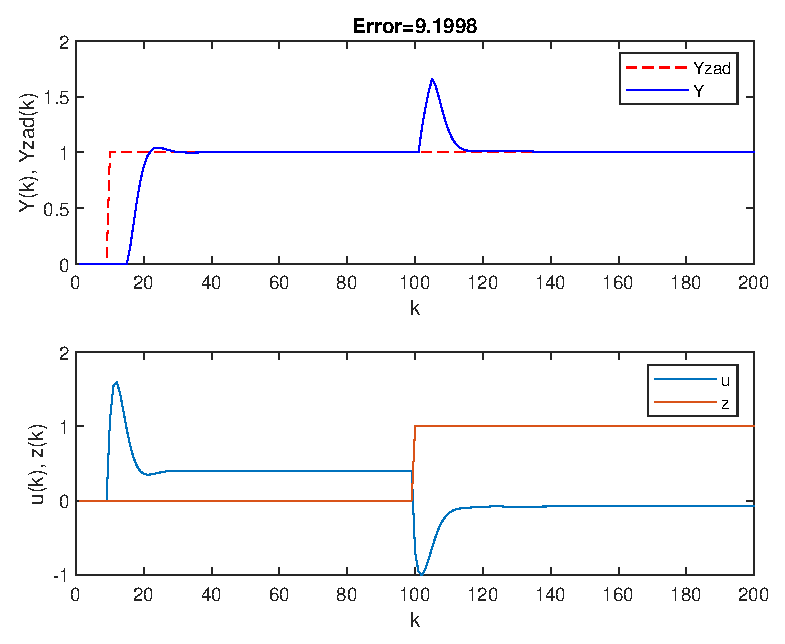
\includegraphics[scale=1]{Rys/zak_bezr.eps}
	\caption{Przebieg bez uwzględniania zakłócenia w regulacji}
	\label{fig:zak_bezr}
\end{figure}